\title{2020/04/10 Discussion}
\author{0616014 楊政道}
\maketitle
\thispagestyle{fancy}
\section{Discussion 1}
\subsection{Based on the requirements, set correct value in the sample code}
\begin{itemize}
    \item 8 samples per measurement
    \item Data Output Rate = 15Hz
    \item Gain=1090(LSb/Gauss)
    \item Convert LSB to Gauss (by using self.scale)
\end{itemize}
\begin{figure}[!h]
    \begin{center}
        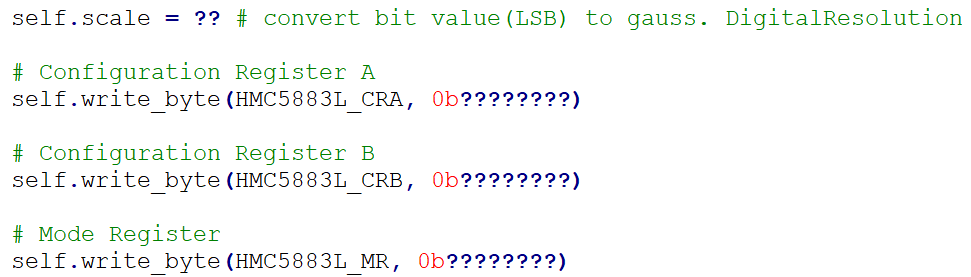
\includegraphics[width=10cm]{d1-1.png}
    \end{center}
\end{figure}
\subsubsection{scale}
\begin{figure}[!h]
    \begin{center}
        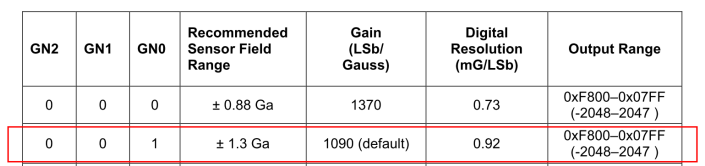
\includegraphics[width=10cm]{d1-1_scale.png}
    \end{center}
\end{figure}
\paragraph{}
Gain = 1090(LSb/Gauss), so the value of the scale is 0.92.
\newpage
\subsubsection{Register A}
\begin{figure}[!h]
    \begin{center}
        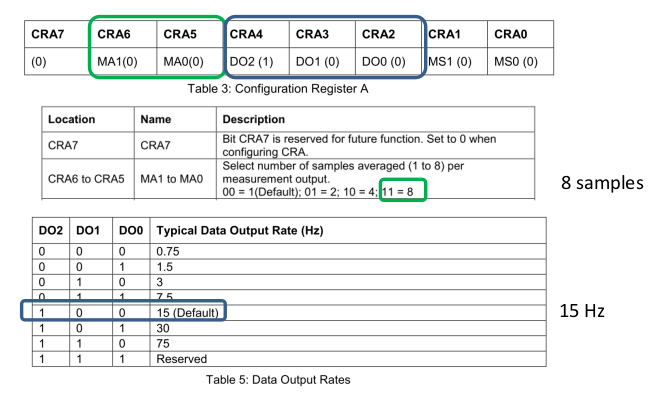
\includegraphics[width=10cm]{d1-1_RA.png}
    \end{center}
\end{figure}
\paragraph{}
8 samples per measurement, Data Output Rate 15Hz, so the value of Register A is 0b00010000.
\subsubsection{Register B}
\begin{figure}[!h]
    \begin{center}
        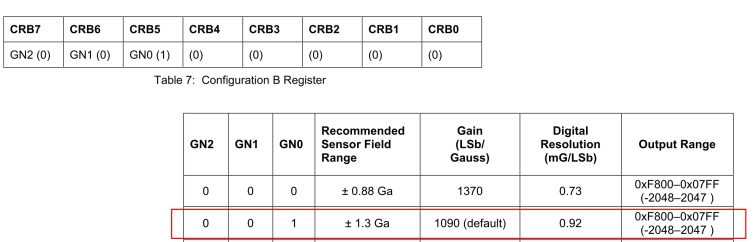
\includegraphics[width=10cm]{d1-1_RB.png}
    \end{center}
\end{figure}
\paragraph{}
Gain = 1090(LSb/Gauss), set the value of Register B to 0b00100000.
\subsubsection{Mode Register}
\begin{figure}[!h]
    \begin{center}
        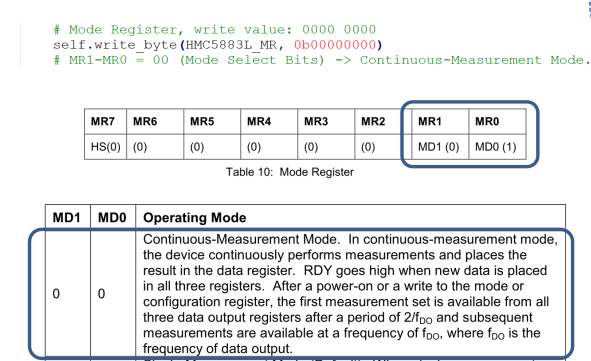
\includegraphics[width=10cm]{d1-1_MR.png}
    \end{center}
\end{figure}
\paragraph{}
Set to thhe continuous mode, so the value of the Mode Register is 0b00000000.
\subsection{Continuously measurement(infinite loop)}
\paragraph{}
In order to make the sensor measure conitnuously, we can put the getValue function of the sensor into a while loop with a time sleep function.
\begin{lstlisting}[language=Python]
while True:
    value = getValue()
    print (value)
    time.sleep(0.1)
\end{lstlisting}
\subsection{Calibrate your sensor (see next page)}
\paragraph{}
In theory, the maximum and minimum value of three axises should be same in absolute value. Therefore, we can spin the sensor first and get the offset value to calibrate it.
\section{Discussion 2}
\subsection{Based on the datasheet, set correct value in the sample code}
\begin{figure}[!h]
    \begin{center}
        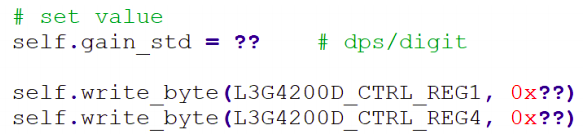
\includegraphics[width=15cm]{d2-1.png}
    \end{center}
\end{figure}
\subsubsection{getPress}
\paragraph{}
According to the datasheet, we need to set the value into 0x34 + (self.oversampling << 6)
\subsubsection{getTempC}
\paragraph{}
According to the datasheet, we need to set the value into 0x2E
\subsection{Continuously measurement(infinite loop)}
\paragraph{}
In order to make the sensor measure conitnuously, we can put the getValue function of the sensor into a while loop with a time sleep function.
\begin{lstlisting}[language=Python]
while True:
    value = getValue()
    print (value)
    time.sleep(0.1)
\end{lstlisting}
